\documentclass[preprint, 3p,
authoryear]{elsarticle} %review=doublespace preprint=single 5p=2 column
%%% Begin My package additions %%%%%%%%%%%%%%%%%%%

\usepackage[hyphens]{url}

  \journal{Transport Geography?} % Sets Journal name

\usepackage{graphicx}
%%%%%%%%%%%%%%%% end my additions to header

\usepackage[T1]{fontenc}
\usepackage{lmodern}
\usepackage{amssymb,amsmath}
% TODO: Currently lineno needs to be loaded after amsmath because of conflict
% https://github.com/latex-lineno/lineno/issues/5
\usepackage{lineno} % add
\usepackage{ifxetex,ifluatex}
\usepackage{fixltx2e} % provides \textsubscript
% use upquote if available, for straight quotes in verbatim environments
\IfFileExists{upquote.sty}{\usepackage{upquote}}{}
\ifnum 0\ifxetex 1\fi\ifluatex 1\fi=0 % if pdftex
  \usepackage[utf8]{inputenc}
\else % if luatex or xelatex
  \usepackage{fontspec}
  \ifxetex
    \usepackage{xltxtra,xunicode}
  \fi
  \defaultfontfeatures{Mapping=tex-text,Scale=MatchLowercase}
  \newcommand{\euro}{€}
\fi
% use microtype if available
\IfFileExists{microtype.sty}{\usepackage{microtype}}{}
\usepackage[]{natbib}
\bibliographystyle{plainnat}

\usepackage{graphicx}
\ifxetex
  \usepackage[setpagesize=false, % page size defined by xetex
              unicode=false, % unicode breaks when used with xetex
              xetex]{hyperref}
\else
  \usepackage[unicode=true]{hyperref}
\fi
\hypersetup{breaklinks=true,
            bookmarks=true,
            pdfauthor={},
            pdftitle={Leveraging GTFS to explore spatial patterns in transit supply with respect to social needs},
            colorlinks=false,
            urlcolor=blue,
            linkcolor=magenta,
            pdfborder={0 0 0}}

\setcounter{secnumdepth}{5}
% Pandoc toggle for numbering sections (defaults to be off)


% tightlist command for lists without linebreak
\providecommand{\tightlist}{%
  \setlength{\itemsep}{0pt}\setlength{\parskip}{0pt}}




\usepackage{subfig}
\usepackage{booktabs}
\usepackage{longtable}
\usepackage{array}
\usepackage{multirow}
\usepackage{wrapfig}
\usepackage{float}
\usepackage{colortbl}
\usepackage{pdflscape}
\usepackage{tabu}
\usepackage{threeparttable}
\usepackage{threeparttablex}
\usepackage[normalem]{ulem}
\usepackage{makecell}
\usepackage{xcolor}



\begin{document}


\begin{frontmatter}

  \title{Leveraging GTFS to explore spatial patterns in transit supply
with respect to social needs}
    \author[Public Transport Research Group (PTRG)]{James Reynolds%
  %
  \fnref{1}}
   \ead{james.reynolds@monash.edu} 
    \author[Public Transport Research Group (PTRG)]{Yanda Qu%
  %
  \fnref{2}}
   \ead{yanda.qu@monash.edu} 
    \author[Public Transport Research Group (PTRG)]{Graham Currie%
  \corref{cor1}%
  \fnref{3}}
   \ead{graham.currie@monash.edu} 
      \affiliation[Public Transport Research Group (PTRG)]{
    organization={Public Transport Research Group (PTRG), Institute of
Transport Studies, Department of Civil Engineering Engineering, Monash
University},addressline={Clayton
Campus},city={Melbourne},postcode={3800},state={Victoria},country={Australia},}
    \cortext[cor1]{Corresponding author}
    \fntext[1]{Research Fellow}
    \fntext[2]{PhD Student}
    \fntext[3]{Professor}
  
  \begin{abstract}
  This is the abstract.

  It consists of two paragraphs.
  \end{abstract}
    \begin{keyword}
    keyword1 \sep 
    keyword2
  \end{keyword}
  
 \end{frontmatter}

\hypertarget{introduction}{%
\section{Introduction}\label{introduction}}

The spatial distribution of transport disadvantage, gaps in transit
supply and accessibility, and related issues have been a focus of
previous research\footnote{See for example \citet{Ricciardi2015}
  \citet{Currie2003Hobart}; \citet{currie2010identifying};
  \citet{Fransen2015Identifying}; \citet{Guzman2017Assessing};
  \citet{Jaramillo2012}; \citet{Preston2007};
  \citet{Delbosc2011Transportproblems}; \citet{Delbosc2011Thespatial};
  \citet{Engels2011Social}; \citet{Pavkova2016};
  \citet{Delbosc2011Using}; \citet{Murray2001};
  \citet{Currie2010Modeling}; \citet{Currie2007Investigating};
  \citet{Currie2007Identifying}; \citet{Yigitcanlar2007};
  \citet{Wu2003}; \citet{Currie2013Exploring};
  \citet{Preston2007Accessibility}; \citet{Hurni2005};
  \citet{Mamun2011}; \citet{El_geneidy2016}; \citet{Kaplan2014};
  \citet{Martens2012}; \citet{Lucas2016AMethod};
  \citet{Liu2012Accessibility}; \citet{Lucas2012Transport_and_social};
  \citet{Lei2010Mapping}; \citet{Mavoa2012GIS};
  \citet{Delmelle2012Evaluating}; \citet{Foth2014Toward};
  \citet{Welch2013Equity}; \citet{Bell2007Travel};
  \citet{Jaramillob2011Urban}; \citet{Guzman2017Assessing};
  \citet{Wee2011Discussing}; \citet{Currie2004Gap};
  \citet{Engels2011Social}; \citet{Litman2002Evaluation};
  \citet{Parolin2017Identifying}; \citet{Xia2016AMulti};
  \citet{Welch2013AMeasure}; \citet{Jang2017Assessing}.}. Much of this
presents methodologies for calculating social needs and transit supply
so as to locate areas where people who most need public transportation
are not getting it. However, such methodologies appear to only rarely be
revisited, reused or otherwise applied to other cases or time periods in
subsequent research. This may in part be because applying an existing
methodology to another location or time period might not generate
sufficient `new' knowledge for publication, and/or be more an activity
for practitioners than for researchers. As well, describing a new
methodology in a research paper might only require presentation of
enough results to demonstrate the concepts, rather than widespread
application to multiple geographic contexts, which might necessitate the
development of software tools to facilitate broader usage.

An example is provided by the \citet{Currie2003Hobart},
\citet{Currie2004Gap}, \citet{Currie2007Identifying},
\citet{currie2010identifying} studies on spatial gaps between the social
need for transport and the supplied transit levels. This work presented
a transit Supply Index (SI) and compared it to measures of social need
for transport across a few Australian cities.\\
But there does not appear to have been much further use of this approach
in research or practice. It is unclear whether the gaps identified in
this previous research have become narrower or being resolved in the
almost two decades since the original analysis. Nor is it clear whether
the identified spatial patterns of transit need, supply and gaps are
generalizable to other places, beyond Hobart
\citep{Currie2003Hobart, Currie2004Gap} and Melbourne
\citep{Currie2007Identifying, currie2010identifying}.\\
This is perhaps in part because at the time it was first published the
data needed to calculate the transit Supply Index (SI) for a particular
location was not typically readily available. The
\citet{currie2010identifying} analysis of Melbourne was based on
combining multiple operator databases and service frequency data that
had been manually extracted from transit agency websites. To apply the
methodology elsewhere would appear likely to have required a bespoke
data collection, cleaning and analysis effort. Nowadays, however, the
General Transit Feed Specification (GTFS) allows timetable data to be
published in a standardized format. More than 10,000 transit agencies
release data this way \citep{GTFS}.

Various tools for analysing GTFS data are now available, but there does
not appear to have been many developed to allow the analysis of spatial
gaps between the social need for transport and the amount of transit
that is supplied. While the previous literature provides a wealth of
methodologies, the availability of tools that might be used by
researchers, practitioners and advocates to use these approaches with
GTFS data relatively easily appears limited.

This gap provides the motivation for the research reported in this
paper, in which a new R package (gtfssupplyindex) specifically developed
to calculate SI scores is presented. The paper also reports results for
Greater Melbourne in 2016 and 2021, matching the most recent censuses
and allowing comparison to the 2006 result reported in
\citet{currie2010identifying}. Comparisons are also made to other parts
of Australia, so as to explore whether findings about Greater Melbourne
are generalizable.

The remainder of this paper is structured as follows: the next section
outlines the background to this research, including the formulation of
the Transit Supply Index (SI), and an explanation of the GTFS. Section 3
then describes the study methodology, followed by presentation of
results in Section 4. Section 5 discusses the results and the
limitations of this study, and outlines directions for future research.
A brief conclusion is provided in Section 6.

\hypertarget{background}{%
\section{Background}\label{background}}

\hypertarget{transit-metrics}{%
\subsection{Transit metrics}\label{transit-metrics}}

Even a brief search reveals many metrics available for benchmarking
transit services. Examples include those in: the extensive Transit
Cooperative Research Program (TCRP) Report 88 guidebook on developing
performance-measurement systems \citep{Ryus:2003aa}; and those used
across benchmarking databases and programs
\citep{Florida-Transit-Information-System:2018aa, UITP:2015aa, Imperial-College-London:2023aa}.
The Fielding Triangle \citep{FieldingGordonJ1987Mpts} provides a
framework for combining indicators of service inputs, outputs and
consumption to describe cost efficiency, cost effectiveness and service
effectiveness. More broadly: \citet{Litman:2003ab} and
\citet{Litman:2016aa} discuss some of the traffic, mobility,
accessibility, social equity, strategic planning and other rational
decision-making-based perspectives underling transport indicators;
\citet{Reynolds:2017ah} extends these into models of how
institutionalism, incrementalism and other public policy analysis
concepts might apply to decision-making processes relating to transit
prioritization; \citet{GuzmanLuisA.2017Aeit}, developed a measure of
accessibility in the context of policy development and social equity for
Latin American Bus Rapid Transit (BRT) networks; and
\citet{Creutzig2020streetspaceallocation} introduced street space
allocation metrics based around 10 ethical principles.

However, many of these, and other, transit metrics may be difficult to
calculate, and/or complex to explain or understand, especially for those
who are not planners, engineers or other technical specialists. Where
pre-calculated metrics are immediately available it may not be possible
for practitioners, researchers or advocates to independently generate
scores so as to test proposed system changes, or demonstrate impacts to
politicans, the general public or others. Contrasting examples are
provided by the metrics in the Transit Capacity and Quality of Service
Manual (TCQSM) and the Transit Score metric \citep{WalkScore:2023tg}.
Transit Scores are readily available on the Transit Score website for
locations with a published GTFS feed. The meaning of these Transit
Scores also appears easy to explain, with the highest possible score of
100 representing the sort of transit accessibility that might be
xperienced in the center of New York. However, the Transit Score
algorithm is a black box, and cannot be calculated independently or
generated for proposed changes to networks. In contrast, the TCQSM
provides a wide range of metrics for measuring different aspects of a
transit system. The TCQSM scores themselves appear easy to understand or
explain, ranging from A (good) to F (bad), and these can be calculated
independently, given sufficient data. \citet{Wong:2013aa} provides an
example of what can be done combining GTFS data with metrics that can be
independently calculating, reporting TCQSM scores across 50 transit
operators.

The GTFS is an open, text-based format, developed originally to allow
transit to be included in the Google Maps navigation platform
\citep{GTFS}. Figure @ref(fig:GTFS\_ERD) shows an Entity Relationship
Diagram (ERD) of the GTFS structure, indicatating how data is stored as
a series of tables (agency, routes, trips etc.) linked by primary and
foreign keys (agency\_id, route\_id, trip\_id etc.). While there are
many software tools for analyzing, visualizing or otherwise manipulating
GTFS data, one to calculate Transit Supply Index (SI) scores is not yet
available.

\begin{figure}
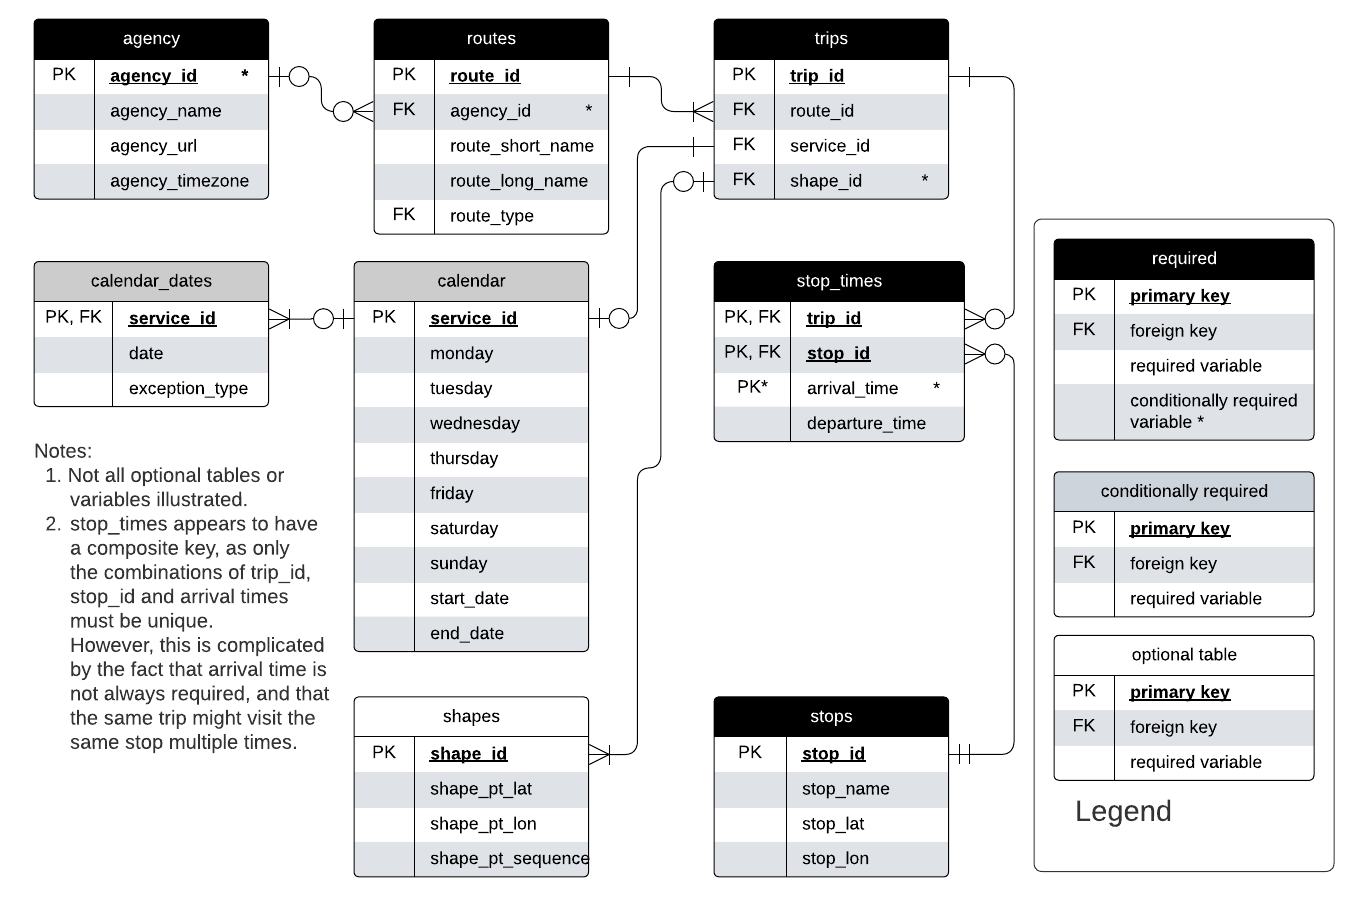
\includegraphics[width=1\linewidth]{graphics/GTFS} \caption{GTFS entity relationship diagram. Source: adapted by author from Alamri et al (2023) and the GTFS Schedule Reference (16/11/2023 revision).}\label{fig:GTFS_ERD}
\end{figure}

\hypertarget{the-transit-suppy-index}{%
\subsection{The Transit Suppy Index}\label{the-transit-suppy-index}}

A generalized form of the SI equation, adapted from
\citet{currie2010identifying}, is:

\[SI_{area, time} = \sum{\frac{Area_{Bn}}{Area_{area}}*SL_{n, time}}\]

where:

\begin{itemize}
\item
  \(SI_{area, time}\) is the Supply Index for the area of interest and a
  given period of time;
\item
  \(Area_{Bn}\) is the buffer area for each stop (n) within the area of
  interest (in \citet{currie2010identifying} this was based on a radius
  of 400 metres for bus and tram stops, and 800 metres for railway
  stations);
\item
  \(Area_{area}\) is the area of the area of interest; and
\item
  \(SL_{n,time}\) is the number of transit arrivals for each stop for a
  given time period.
\end{itemize}

\begin{figure}
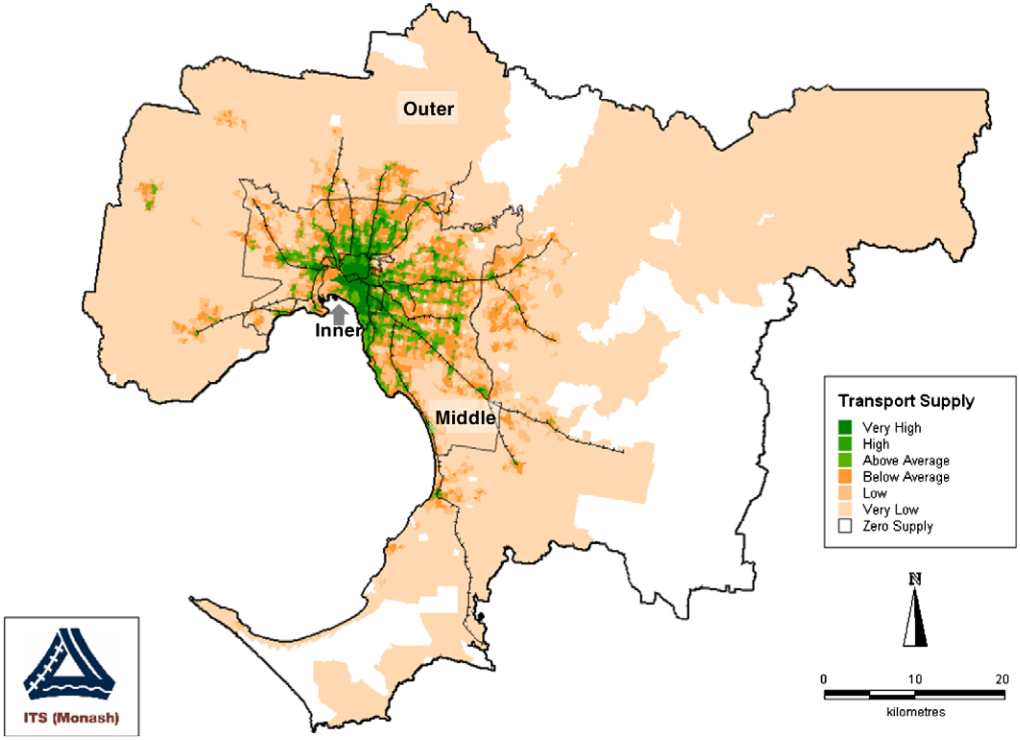
\includegraphics[width=1\linewidth]{graphics/Currie2010SI} \caption{Distribution of supply measure scores – Metropolitan Melbourne (2006), Source: Currie (2010)}\label{fig:Currie_map_SI}
\end{figure}

\citet{currie2010identifying} reported SI scores across Greater
Melbourne in 2006, as shown in Figure \ref{fig:Currie_map_SI}. The
general patterns appear to be higher levels of transit supply in the
middle and inner suburbs and along passenger railway lines. Outer areas
tend to have very low SI scores or no transit supply at all.

\hypertarget{social-need-and-needs-gap}{%
\subsection{Social need and needs gap}\label{social-need-and-needs-gap}}

As well as measuring transit supply, \citet{currie2010identifying} also
assessed the social need for transit across Greater Melbourne using: the
Australian Bureaus of Statistics' Index of Related Socio-Economic
Advantage/Disadvantage (IRSAD); a transport needs index derived by
\citet{currie2010identifying} from eight weighted indicators; and a
combination of the two. Figures \ref{fig:Currie_chart_gap} and
\ref{fig:Currie_map_gap} reproduce the resultant chart and map combining
needs and supply to identify gaps.

\begin{figure}
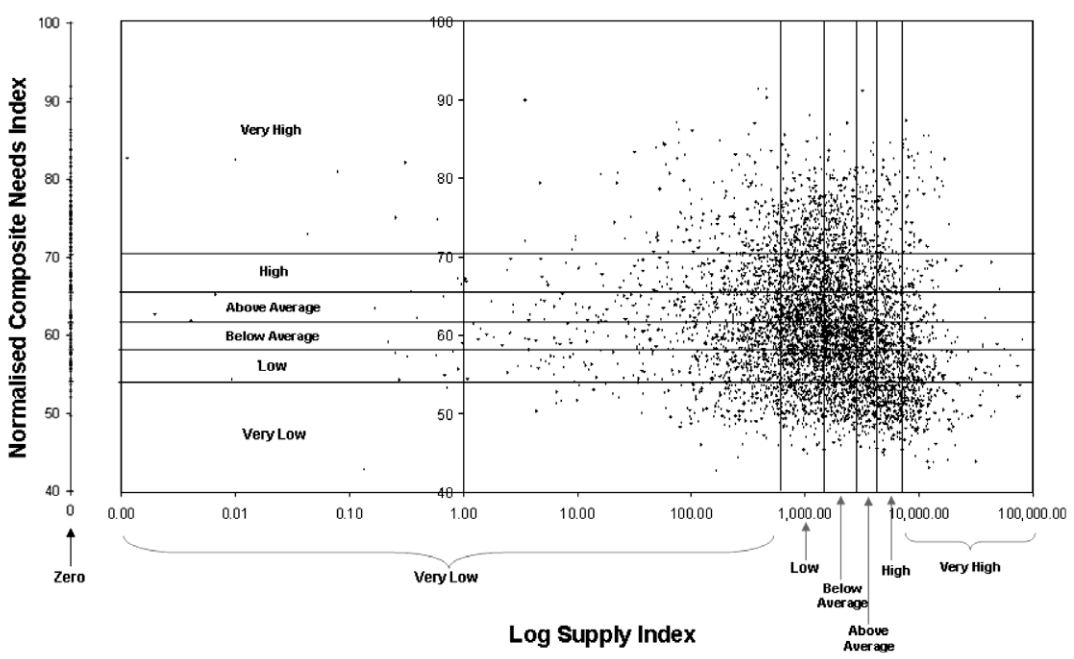
\includegraphics[width=1\linewidth]{graphics/Currie2010chart} \caption{Log supply score and need index values – Melbourne needs-gap study, Source: Currie (2010)}\label{fig:Currie_chart_gap}
\end{figure}

\begin{figure}
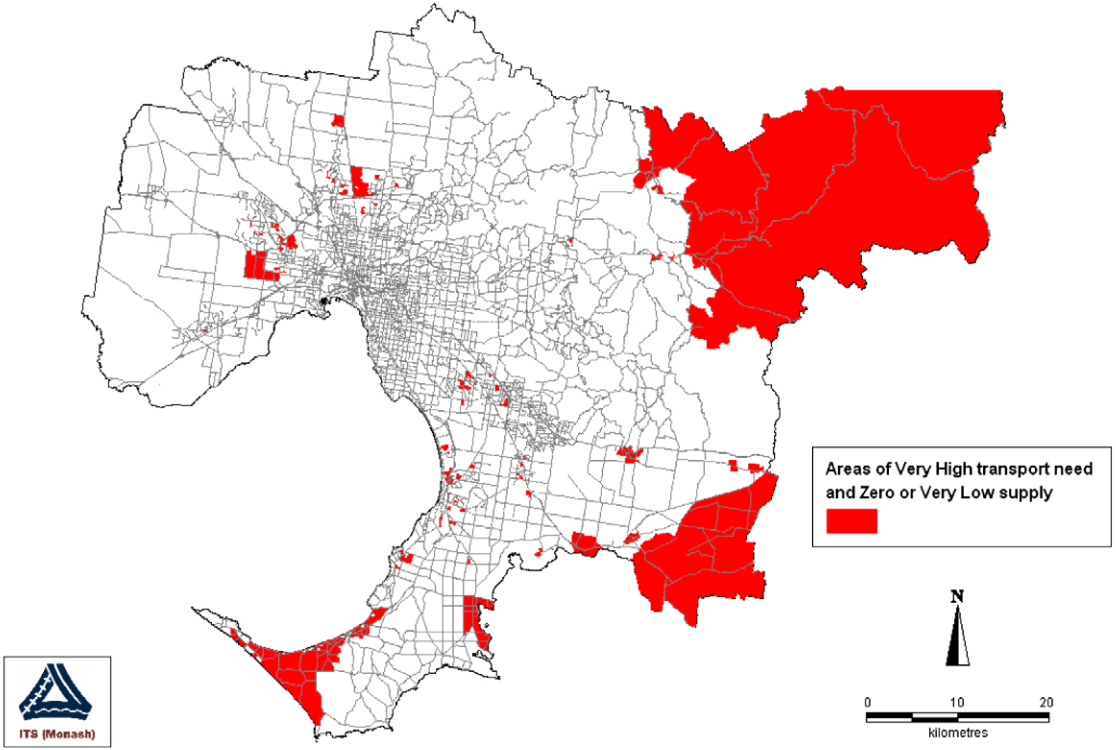
\includegraphics[width=1\linewidth]{graphics/Currie2010gap} \caption{Melbourne needs-gap – very high transport need areas with zero or very low public transport supply, Source: Currie (2010)}\label{fig:Currie_map_gap}
\end{figure}

The results indicated service gaps of concern, especially in outer parts
of Melbourne where low density development patterns make provision of
transit more challenging. \citet{currie2010identifying} found that
``(o)verall, 8.2\% of Melbourne residents have `very high' needs but
`zero', `low' or `very low' public transport supply.''\\
They also suggested that planning for transit service provision using
this approach would be ``substantially more useful than the presentation
of anecdotal evidence, which is the most common means of identifying
transport needs in local transport studies throughout the world.''
However, it doesn't appear that this approach has been widely adopted in
practice or academia. Our suspicion is that while the SI has a
relatively simple formula and requires only geographic and timetable
data, the lack of a software tool to perform these calculations may be
part of the reason that it has not been more widely adopted and why
formal needs-supply-gap analysis may still be uncommon.

It is also unclear whether the patterns in Melbourne identified in
\citet{currie2010identifying}, where areas with very high transport
needs but zero or very low transit supply tend to be in outer areas
serviced by buses, are similar to patterns in other cities. Nor is it
clear whether the patterns in Melbourne itself have changed since the
2006 analysis. Developing a software tool to calculate SI tools from
GTFS data, and then using it to comparing current conditions and other
locations to the findings of \citet{currie2010identifying}, therefore,
is the primary aim of this paper.

\hypertarget{methodology}{%
\section{Methodology}\label{methodology}}

This study developed a package of tools for calculating the SI from GTFS
data using the R programming language \citep{R-base}. The
recommendations of \citet{wickham2023r} informed the package setup and
development approach. Various existing packages were relied upon
including: the sf package \citep{R-sf} for geospatial analysis; the
tidyverse \citep{tidyverse2019}; gtfstools \citep{R-gtfstools}; and
tidytransit \citep{R-tidytransit}. Australian Bureau of Statistics (ABS)
data was also used, sourced via the strayr and absmapsdata packages
\citep{r-strayr}. Some code was adapted from examples, vignettes and
other documentation in these and other packages.

Two cases were used during the code development and testing, such that
results might be generated for real GTFS data: the Mornington Peninsula
Tourist Railway GTFS feed; and the Public Transport Victoria (PTV) GTFS
feed, both in Victoria, Australia. Both were selected primarily for
convenience, given that the authors are familiar with the typical
service patterns and geography. Adopting the Mornington Peninsula
Tourist Railway network, which consists of only three stations, also
facilitated hand calculation of the SI as a cross-check of the results
produced by the developed package.

Figure @ref(Melbourne\_map)) shows the areas of interest relevant to the
code development and testing, and selected railway stations. Statistical
Area (SA) zones were adopted from the Australian Bureau of Statistics
\citep{ABSmaps} as the areas of interest, and included SA3
zones\footnote{These are generally similar to Local Government Area
  (LGA) boundaries.} across the Greater Melbourne Greater Capital City
statistical area (Figure @ref(Melbourne\_map), left); and SA1
zones\footnote{SA1 zones are the smallest geographical areas for which
  results are reported in the Australian census.} within 800 metres of
the Mornington Penninsula railway (Figure @ref(Melbourne\_map), right).

\begin{figure}
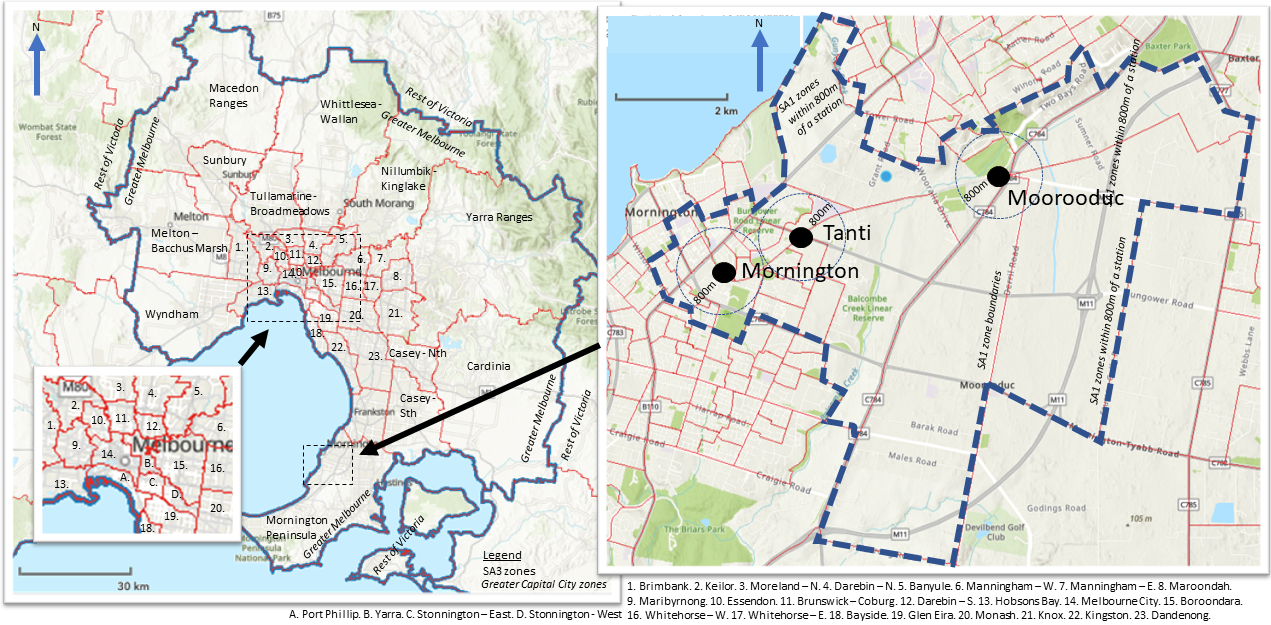
\includegraphics[width=1\linewidth]{graphics/all_maps} \caption{Areas of interest}\label{fig:Melbourne_map}
\end{figure}

\hypertarget{mornington-penninsula-tourist-railway}{%
\subsection{Mornington Penninsula Tourist
Railway}\label{mornington-penninsula-tourist-railway}}

The Morning Peninsula Tourist Railway is in the outer south-east of
Melbourne, running on Sundays and Wednesdays between Mornington and
Moorooduc, with an intermediate stop at Tanti Park\footnote{see
  https://transitfeeds.com/p/mornington-railway/806/latest/stops}. A
GTFS feed from 2018 was selected for the purposes of tests, and for
demonstrating the code and outputs reported here.

\hypertarget{public-transport-victoria-ptv}{%
\subsection{Public Transport Victoria
(PTV)}\label{public-transport-victoria-ptv}}

The Victorian GTFS feed, published by Public Transport Victoria (PTV)
and with historical feeds sourced via
\citet{transitfeeds_victoria:2023aa}, was used for analysis of Greater
Melbourne and Victoria. SI scores were obtained for the weeks starting
on the day of the census in 2016 and 2021, which were on Tuesday 9th and
10th of August respectively.

\hypertarget{results}{%
\section{Results}\label{results}}

\hypertarget{code-structure-and-functionality}{%
\subsection{Code structure and
functionality}\label{code-structure-and-functionality}}

Developed code is available and documented on github (see
\citet{gtfssupplyindex_github}). The structure of the package, functions
developed, and data tables are shown in Figure @ref(fig:SI\_ERD), which
indicates how the package takes input from three files: a gtfs feed
(gtfs.zip); a sf object describing the geometry of the areas of interest
for which the SI is to be calculated; and a csv file (included in the
package) defining the buffer zone distances for each route type. The
ultimate output is a si\_by\_area\_and\_hour table (Figure
@ref(fig:SI\_ERD), bottom-right), which reports the SI score for each
hour of a day specified by the user.

\begin{figure}
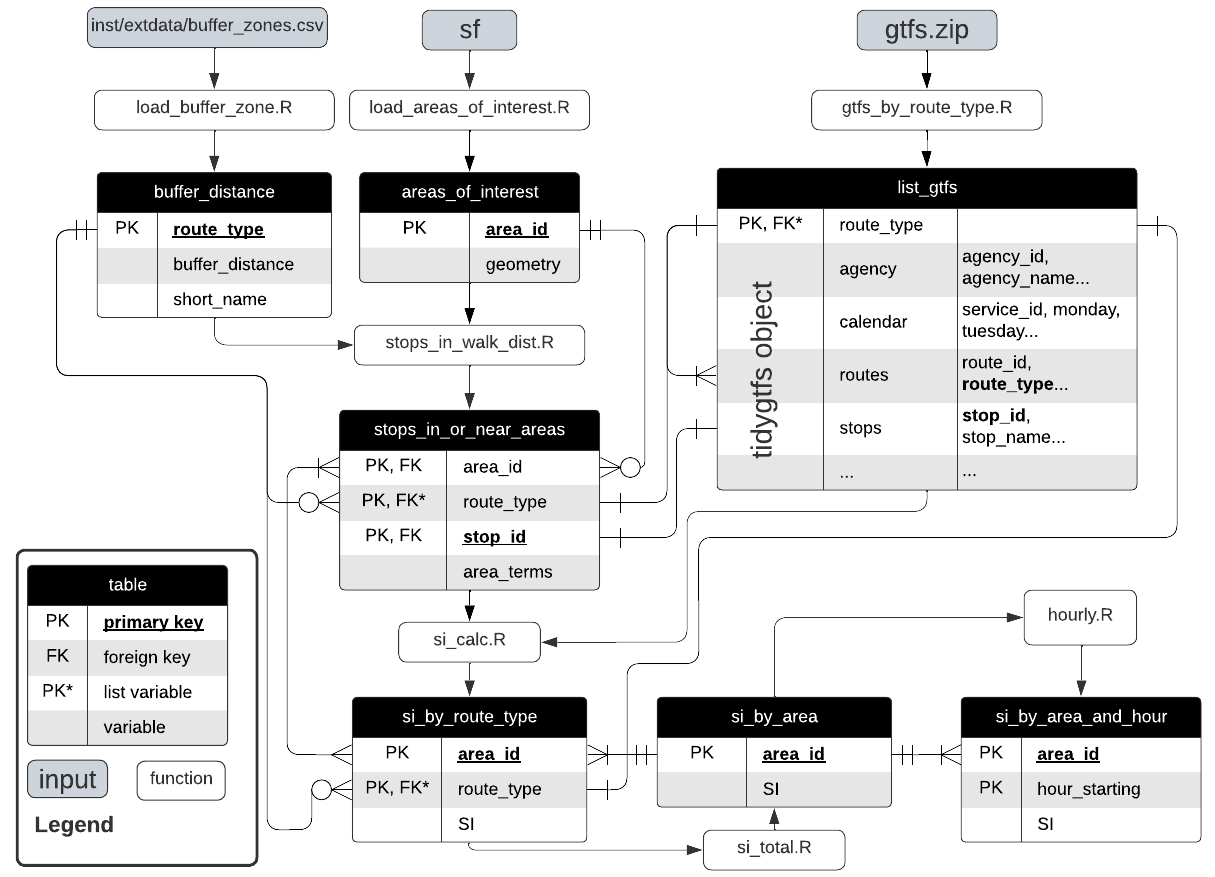
\includegraphics[width=1\linewidth]{graphics/SI_data_structure} \caption{Entity Relationship Diagram (ERD) showing the data structure and functions related to the gtfssupplyindex package}\label{fig:SI_ERD}
\end{figure}

The various functions included in the package and their output are
explained in the following, using the Mornington Peninsula GTFS as a
worked example\footnote{This paper itself was prepared in Rmarkdown and
  is available at
  https://github.com/James-Reynolds/gtfssupplyindex\_main\_paper. Code
  snippets used to produce the outputs of the worked example can be
  viewed there.} Individual steps are:

\begin{enumerate}
\def\labelenumi{(\arabic{enumi})}
\item
  loading the gtfs.zip file: the gtfs\_by\_route\_type function loads
  the gtfs data and splits it into a list (by route\_type) of tidygtfs
  objects, using the filter\_by\_route\_type function from the gtfstools
  package \citep{filter_GTFS_by_mode}.
\item
  loading geometry information about the areas of interest: geographical
  data about the areas of interest are loaded by the
  load\_areas\_of\_interest function into an sf object, using the sf
  package \citep{R-sf}. The resultant areas\_of\_interest table contains
  each area\_id and its associated geometry. Data about buffer zones,
  specifically the walking distance threshold assigned to each
  route\_type (mode) is then loaded, again through another function
  (load\_buffer\_zone).
\item
  calculating which stops are within the catchment walking distance of
  which areas: using the stops\_in\_walk\_dist function. Figure
  @ref(fig:calculate\_stop\_in\_or\_near\_areas\_verbose)) shows how
  this function identified SA1 areas within the 800 metre catchment of
  the three Mornington stations.
\end{enumerate}

\begin{figure}
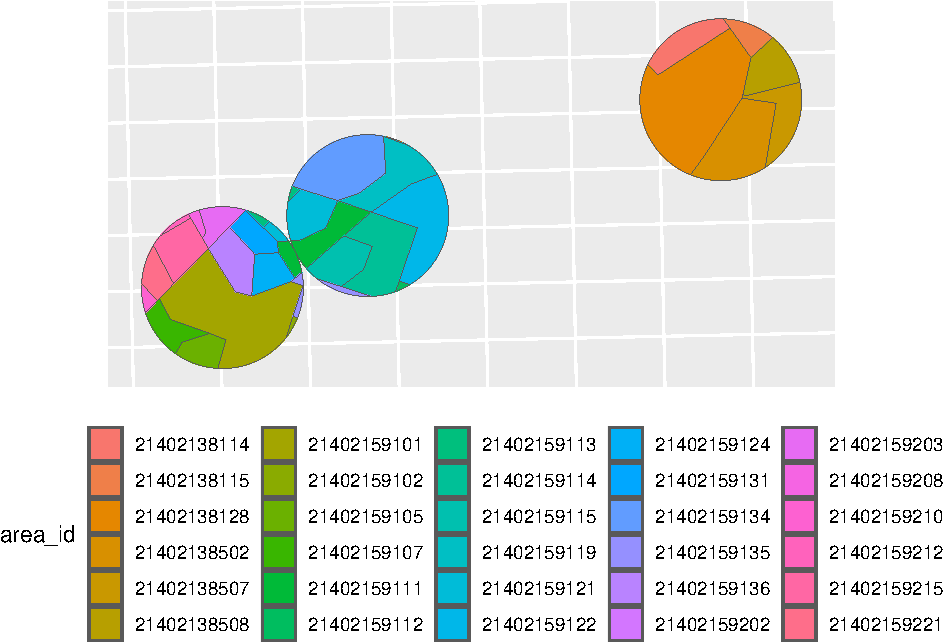
\includegraphics[width=1\linewidth]{Leveraging_GTFS_to_assess_transit_supply_Transport_Geography_files/figure-latex/calculate_stop_in_or_near_areas_verbose-1} \caption{Step 3, stop catchments for the Mornington Penninsula Tourist Railway, showing intersections with SA1 zones}\label{fig:calculate_stop_in_or_near_areas_verbose}
\end{figure}

\begin{enumerate}
\def\labelenumi{(\arabic{enumi})}
\setcounter{enumi}{3}
\tightlist
\item
  Calculating SI scores for a given time period: The si\_calc.R function
  calculates the number of arrivals in a given time period, using code
  adapted from an article included in the tidytransit package
  \citep{tidytransit_departure_timetable}, and combines this with the
  calculated area components. The si\_total.R and hourly.R functions
  provided aggregation, giving the results mapped in Figure
  @ref(fig:SI\_mornington\_20181230\_output).
\end{enumerate}

\begin{figure}
\centering
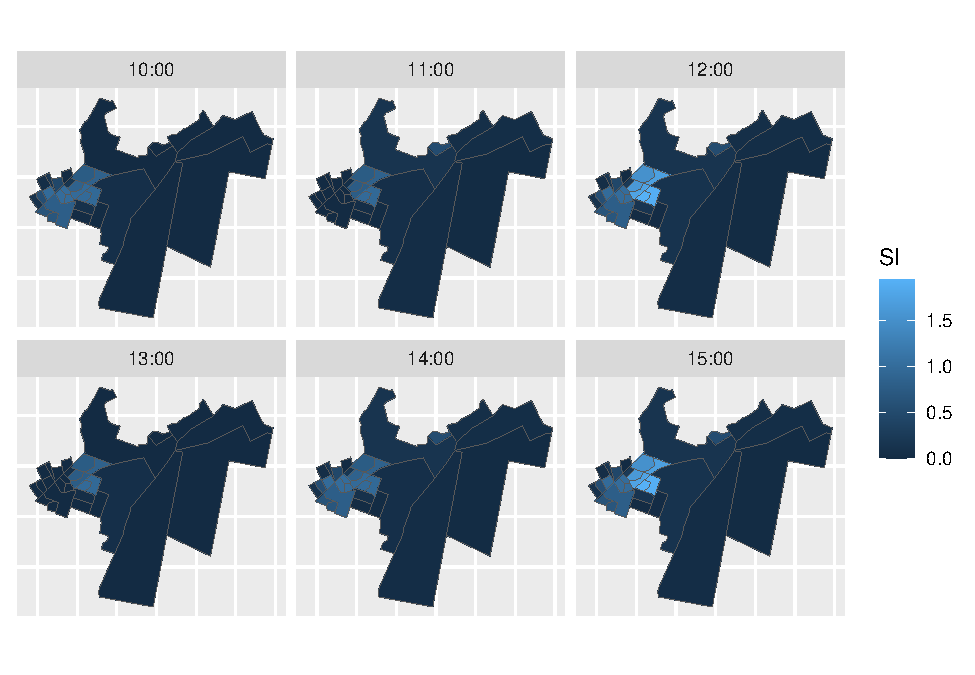
\includegraphics{Leveraging_GTFS_to_assess_transit_supply_Transport_Geography_files/figure-latex/SI_mornington_20181230_output-1.pdf}
\caption{Mornington Penninsula Tourist Railway hourly SI values for
December 30, 2018}
\end{figure}

\hypertarget{si-scores}{%
\subsection{SI scores}\label{si-scores}}

\begin{figure}
\centering
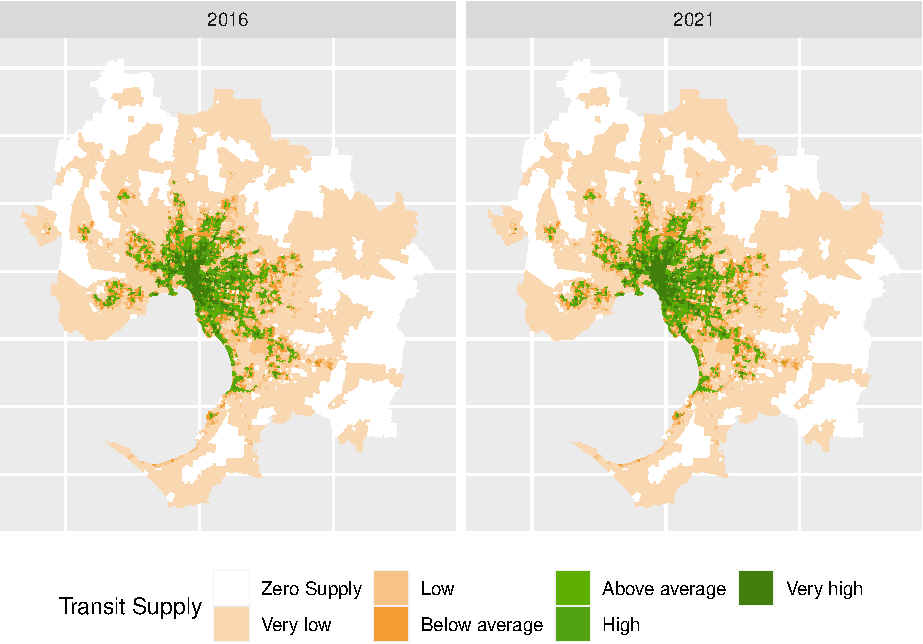
\includegraphics{Leveraging_GTFS_to_assess_transit_supply_Transport_Geography_files/figure-latex/Greater_Melbourne_2016_2021-1.pdf}
\caption{SI scores, census day 2016 and 2021}
\end{figure}

\hypertarget{imrad}{%
\subsubsection{IMRAD}\label{imrad}}

\hypertarget{comparing-cases}{%
\subsection{Comparing cases}\label{comparing-cases}}

\hypertarget{population-and-equality}{%
\subsubsection{Population and equality}\label{population-and-equality}}

\hypertarget{purpose-of-transit-in-the-citys-transport-policy}{%
\subsection{Purpose of transit in the city's transport
policy}\label{purpose-of-transit-in-the-citys-transport-policy}}

\hypertarget{indexes-and-comparing-cities}{%
\subsection{Indexes and comparing
cities}\label{indexes-and-comparing-cities}}

\hypertarget{discussion}{%
\section{Discussion}\label{discussion}}

\hypertarget{limitations}{%
\subsection{Limitations}\label{limitations}}

\hypertarget{directions-for-furture-research}{%
\subsection{Directions for furture
research}\label{directions-for-furture-research}}

\hypertarget{conclusions}{%
\section{Conclusions}\label{conclusions}}

\renewcommand\refname{References}
\bibliography{References.bib, packages.bib}


\end{document}
